\chapter{MM-quecat}
\label{quecat}

In the previous two chapters, we introduced MMQL, as well as the supporting algorithms enabling its implementation.
However, we presented both on a theoretical level only.
To properly evaluate the validity and correctness of our proposal, it must be verified in practice by way of implementation.
Therefore this chapter presents \textit{MM-quecat}\footnote{\url{https://github.com/yawnston/querycat}}, a proof-of-concept implementation of the core concepts of MMQL.
The purpose of this implementation is the verification of our proposed approach. Full implementation of all MMQL concepts for all scenarios would be beyond the scope of this thesis, which is why the implementation focuses only on the key parts of MMQL.
This chapter not only describes the implementation of MM-quecat itself, but also the technical challenges faced along the way.

\section{Solution Architecture}

MM-quecat is a Python 3\footnote{\url{https://www.python.org/}} library which provides the functionality of executing MMQL queries.
Its interface is rather simple on the surface - it provides a function \texttt{execute\_query}, which takes the input query as a string, and returns an instance category (see~\cref{categorical:section:instance}) representing the result of the query.

To do this, it needs to communicate with MM-evocat~\cite{evocat}, which is a multi-model data modeling and evolution framework based on category theory, written as a Java server application.
MM-evocat has the functionality of creating a schema category (see~\cref{categorical:section:schema}).
For that reason, MM-quecat's main interface function \texttt{execute\_query} also contains a parameter containing the ID of the schema category, which refers to a schema category within MM-evocat.
In MM-evocat, one can not only model the schema category, but also create the mappings necessary to transform data from its native representation into the categorical representation, using an algorithm for model-to-category transformation~\cite{unified_representation}.
While including MM-evocat in the solution does introduce overhead in the form of network communication, the benefits it brings outweigh the negatives for our purposes, since it includes the categorical modeling tools which are necessary for MM-quecat to do its job.
Without MM-evocat, MM-quecat would need to implement all of the necessary functionality itself, effectively duplicating the functionality of MM-evocat to avoid network overhead, which is not desirable at this point of the tool's lifecycle as proof-of-concept software.
MM-evocat is also still in active development by its author and is not yet fully finished, which further complicates its usage, as we will mention again going forward in this chapter.
Perhaps in the future, if the a full and optimized implementation of MM-quecat is desired and when MM-evocat's development is finished, both tools could be merged into a single one.

\begin{figure}[h]
\centering
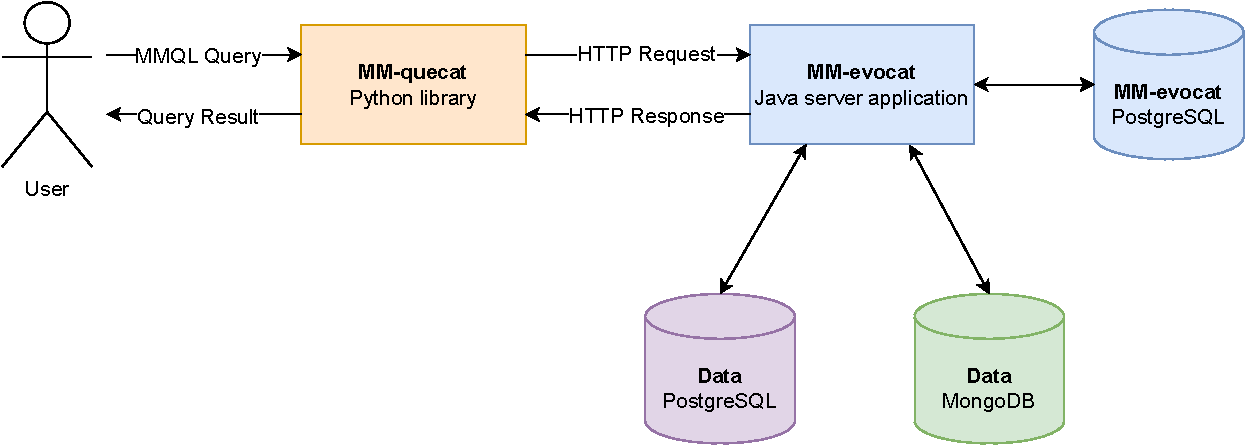
\includegraphics[width=\textwidth]{img/quecat-architecture.pdf} 
\caption{Architecture of the MM-quecat solution.}
\label{fig:quecatarchitecture}
\end{figure}

The architecture of the whole solution can be seen in~\cref{fig:quecatarchitecture}, which shows MM-quecat communicating with MM-evocat via HTTP.
We can see that MM-quecat sends requests to an instance of MM-evocat which contains the necessary schema category and mappings representing the data being queried, as well as maintaining the connections to the relevant databases.
Note that at no point does MM-quecat actually need to communicate with the queried databases directly, as the queries generated by MM-quecat are passed to MM-evocat, which executes the queries and transforms their results to the categorical representation using a mapping provided by MM-quecat\footnote{While direct database communication is not necessary in MM-quecat's current form, the implementation of a fully-featured multi-model query planner would necessitate this direct connection, as the query planner would need access to the databases' own query planners, usually in the form of a database explain command, to assess the cost of MMQL multi-model query plans.}.
This increases the modularity of the solution, as MM-quecat only needs to rely on the categorical interface of MM-evocat, and the database wrappers (recall~\cref{algorithms:subsection:wrappers} where we introduced the notion of database wrappers) have their implementation greatly simplified, as they only need to generate the native queries without having to worry about executing them, or transforming their results to a categorical representation\footnote{A potential problem may arise if the database wrappers need to access the database interface to query it for the supported query language version in cases where the database wrapper is deciding whether it may use a newer language feature. However, this would be solved by simply adding the database connection to MM-quecat just like in the case of the query planner.}.
Lastly,~\cref{fig:quecatarchitecture} shows that MM-evocat also has its own PostgreSQL database which it uses to store schema and mapping data, as well as instance categories.
This database is separate from the databases containing the actual data being queried.
Going forward, MM-quecat will also be wrapped in a simple HTTP API as required for the purposes of the querying tool which we will introduce in~\cref{querytools}, as this querying tool will continue being worked on as part of a conference demo paper which the author of this thesis is co-authoring~\cite{mm_quecat}.

For completeness, we should also mention the choice of Python as the language for the implementation of MM-quecat.
The ecosystem of tools developed for multi-model data representation at the Faculty of Mathematics and Physics of Charles University, which MM-quecat and MM-evocat are a part of, already contains projects in both Java and Python, making both languages natural candidates for the cohesion of the tool ecosystem.
From these two languages, Python was chosen due to the personal preferences of the author of this thesis, as they have extensive experience with Python, but little to no Java experience.
To add to this, it is the author's personal belief that Python, with its simplicity, ease of use and universal usefulness, is the language of the future, and will continue to gain market share while Java slowly fades away to make room for more modern languages.

Since MMQL is a multi-model query language and MM-quecat is a library implementing MMQL, we also need to discuss MM-quecat's multi-model capabilities.
As implemented, MM-quecat supports two models - relational in the form of PostgreSQL, and document in the form of MongoDB.
The reason for this is relatively straightforward, as both databases are among the most popular in their class, and together they represent a significant market share of the database space.
In addition, MM-evocat currently only supports these two databases, which means that MM-quecat cannot support additional databases without their corresponding implementation in MM-evocat.
Among other limitations, MM-evocat only supports string values, meaning the data type of everything in MM-evocat is a string.
For this reason, MM-quecat is also constrained to only supporting strings, even though MMQL also supports other data types.

With the solution architecture out of the way, we will describe specific parts of MM-quecat and their implementation, loosely following the solution structure proposed in~\cref{algorithms:section:approach}.

\section{Parsing}

The first step in implementing any language, be it a query or programming language, is to implement a parser for this language.
This is because it is not feasible to work with a language based on its raw text alone, but rather it is more practical to operate on language-level constructs which are parsed from the raw text by a parser.
While the parser for MMQL could be manually implemented, a smarter solution exists in the form of parser generators.
These tools generally accept some sort of formal grammar as input, and in return generate a parser for the language represented by the grammar.
As it happens, we had been planning to formally specify the grammar of MMQL anyway, which made using the grammar to generate a parser a natural step.
The grammar used to generate the parser for MM-quecat is included  in~\cref{attachment:grammar}.

This was accomplished using the ANTLR\footnote{\url{https://www.antlr.org/}} library, which is a parser generator for reading, processing, executing, or translating structured text or binary files.
ANTLR was used to generate the parser classes in Python, at which point we implemented an abstract syntax tree (AST) visitor, which walks the AST created by the generated parser, and converts it into a suitable form for further processing in the query execution process.
This form consists of translating the input graph patterns into sets of triples, coupled with additional constructs such as \texttt{FILTER} expressions or other query features.

\section{Creating Query Plans}

As described in~\cref{algorithms}, we need to divide the query up into query parts to form query plans.
First, queries are preprocessed to transform triples containing compound morphisms into multiple triples, each containing a base morphism.
For each point where a compound morphism was split, a temporary internal variable is inserted into the query.
As discussed in~\cref{algorithms:subsection:preprocessing}, this greatly simplifies query processing as a whole, but introduces issues when it comes to performance and recursive paths.
The performance consideration is not an issue for MM-quecat, as achieving high performance is not within the scope of its proof-of-concept nature (and within the scope of this thesis in general).
The consideration of recursive morphisms, while unpleasant, is also not key to demonstrating the viability of MMQL and MM-quecat as a whole.
The implementation of recursive morphisms would also be rather complex, which is why they are not supported in the implementation, giving us space to focus on the main focus points of this thesis.

Aside from the preprocessing, the implementation of query plan creation largely copies the algorithm outlined in~\cref{algo:subsection:queryplan}, which is why we will not discuss it here further.

\section{Query Translation}

The query translation algorithm is a simplified, limited version of the algorithm presented in~\cref{algo:subsection:translation}, supporting simple queries with both base and compound morphisms.
However, the scope of the implementation of this algorithm is not limited only by the implementation effort required.
As we mentioned earlier in this chapter, MM-evocat is still undergoing active development by its author, and as a consequence, some of its features are not quite finished yet.
For example, there is an issue where if MM-quecat generates queries requiring database joins on multiple kinds (like multiple tables in the relational model or multiple collections in the document model), MM-evocat will not correctly process these queries when translating their results into the categorical representation, yielding an incorrect instance category.
For this reason, MM-quecat cannot support queries with multiple kinds in a single query part at this time.
While this is bothersome in terms of the completeness of the implementation, it is not an issue in the scope of a proof-of-concept implementation, as we can demonstrate the multi-model capabilities of MM-quecat on multi-model queries which do not require the use of multiple kinds from the same database.
One such query is later shown in~\cref{fig:evalmultimodelmmql} while evaluating the weaknesses of MM-quecat.

\section{Selecting the Best Query Plan}

In~\cref{algo:subsection:bestplan}, we discussed the difficulties which come with multi-model query planning, and the lack of related work on the subject, with most sources only considering single-model query planning within the context of a single database.
For that reason, in~\cref{algo:subsection:bestplan} we left the selection of the best query plan as an open point which is beyond the scope of this thesis, which already breaches the vast and complex area of multi-model querying with little related work to use as a base.
Therefore in MM-quecat, the implementation of best plan selection is purposefully very basic - an arbitrary query plan is selected if multiple plans are present due to data redundancy.
The implementation of a more sophisticated selection process first necessitates additional research on possible approaches to this problem.

\section{Query Execution}

As discussed earlier in this chapter, MM-evocat has the ability to execute native database queries in PostgreSQL and MongoDB, and then transform their results into the categorical representation.
It also has the ability to merge the results of multiple such queries over the same schema category into a single instance category, using the objects' identifiers to determine the proper way to join the data.
However, MM-evocat does not have the ability to execute arbitrary queries as required by MM-quecat, and its capability is limited to trivial projection-only queries that exactly copy the structure of the defined mappings.
This is an issue, because MM-quecat generates various queries, which then need to be executed against the databases.

Because MM-evocat is in active development, waiting for MM-evocat to support this arbitrary query execution was not realistic within the context of this thesis.
This is why MM-quecat is actually using a modified instance of MM-evocat\footnote{\url{https://github.com/yawnston/evolution-management}}, which was forked from the main implementation, in which the author of this thesis has made the modifications necessary for MM-quecat to fully function.
The modifications include, but are not limited to:

\begin{itemize}
    \item Modifying the API to allow execution of arbitrary database queries;
    \item Modifying the database wrappers for PostgreSQL and MongoDB to execute the provided queries, including the ability for the MongoDB wrapper to execute aggregation pipelines instead of simple find queries;
    \item Modifying the API to allow the retrieval of instance morphisms, in addition to the retrieval of instance objects, which was already implemented; and
    \item Addition of Docker\footnote{\url{https://www.docker.com/}} configuration files to easily run MM-evocat, since its setup is not very straightforward and includes multiple components.
\end{itemize}

For this reason, MM-quecat only functions with the modified version of MM-evocat.
However, in the future, when MM-evocat is modified by its author to fully support the features required by MM-quecat, these temporary modifications will become obsolete, and MM-quecat will use the main, up-to-date MM-evocat.

Aside from the necessity for these modifications, the query execution algo\-rithm operates mostly as described in~\cref{algorithms}.
MM-quecat uses the API provided by MM-evocat to create a copy of the queried schema category, and to define the mappings which are needed by the query parts in the query.
These mappings define the shape of the results of each individual native database query, effectively telling MM-evocat how to transform the result of this query into the categorical representation.
The queries generated by MM-quecat are executed within MM-evocat, including joining of their results into a single instance category.
This instance category is then retrieved from MM-evocat using the modified API, and the remaining steps are executed as described in~\cref{algorithms}, projecting the instance category to the final instance category, along with creating the schema category defining this result instance category.
The final instance category is then returned as the result of the query.

Note that in our description of the proposed approach in~\cref{algorithms:section:approach}, we also mentioned the need to transform the query result into a more usable representation, such as JSON.
We discussed this in greater detail in~\cref{algo:subsection:transform}, where we mentioned the fact that we can use an existing algorithm for category-to-model transformation~\cite{unified_representation}.

This is another limitation where MM-evocat is not quite ready, as this functionality is not yet fully implemented as required by MM-quecat\footnote{In particular, the algorithm for category-to-model transformation itself is implemented, but not the relevant functionality for the transformation to a format like JSON or RDF.}.
However, when the required functionality is complete on the side of MM-evocat, MM-quecat will take the schema category corresponding to the query result, define the required mappings to transform the result into a JSON representation, and send both over to MM-evocat to perform the actual transformation.

As a whole, the implementation of MM-quecat in this form is sufficient to verify the validity of our proposed approach, as we later demonstrate in~\cref{eval} with concrete queries processed by MM-quecat.
However, as can be seen from the solution architecture, there is certainly room for performance optimization, since there is quite a bit of network communication overhead between MM-quecat and MM-evocat, along with the proposed algorithms being optimized for readability and simplicity, not performance.
These considerations will also be discussed in~\cref{eval}.
